\begin{problem}{/images/problems/pic.jpg}{Dragons on the Chess Board}Dragon is a special chess piece that can move to the cells specified in the picture.

How many ways can 3 dragon pieces be placed on an $8\times8$ chessboard in a way that no two can move to each other's places in one step.

\begin{center}
	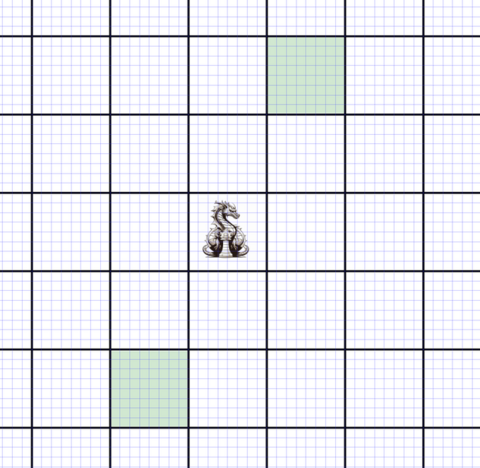
\includegraphics[width=9cm]{/images/problems/42_dragon.png}
\end{center}


Link to the problem on Twitter:  \url{https://twitter.com/Riazi_Cafe/status/1706574099131302222}\end{problem}
\begin{solution}
The answer to the question is equal to 39084.\\[0.2cm]

To show this, we divide the $8 \times 8$ table into 22 chains as follows (the color of the cells in each chain is the same).

\begin{center}
	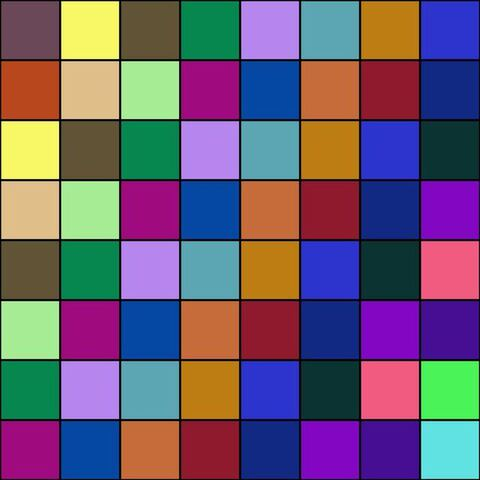
\includegraphics[width=9cm]{/images/problems/42_diagram0.jpg}
\end{center}

Two dragons threaten each other if they are placed in a chain next two each other.
The number of chains of length 4 is equal to 10, and the number of chains of length 3, 2, and 1 is equal to 4.

Next, we count the number of configurations wherein at least two dragons threaten each other (can move to each other's places in one step). These configurations can be divided into 3 categories:

\begin{enumerate}
\item All three dragons are in a chain and two pairs of them threaten each other.
\item All three dragons are in a chain, but only one pair of them threaten each other.
\item A pair of dragons threaten each other and the third dragon is in a different chain.
\end{enumerate}

The number of configurations of category 1 is equal to $10 \cdot 2 + 4 = 24$ (two for each chain of length 4 and 1 for each chain of length 3).
The number of configurations of category 2 is equal to $20 \cdot 10 = 20$ (two for each chain of length 4).
The number of configurations of category 3 is equal to $3 \cdot 10 \cdot 60 + 2 \cdot 4 \cdot 61 + 1 \cdot 4 \cdot 62 = 2536$.
Thus the total number of configurations wherein at least two dragons threaten each other is equal to $2536 + 20 + 24 = 2580$.

The total number of configurations that three dragons can be placed on the table is $\binom{64}{3} = 41664$.
Therefore, the answer is equal to $41664 - 2580 = 39084$.
\end{solution}
